\section{Results}\label{sec:results}

We collected the snapshot on 23 July 2026. Of the $448$ app$\times$country cells,
we obtained a definitive availability signal for \textbf{all 448 (100\% coverage)}
after excluding Iran, which has no Apple storefront. Across the snapshot, 49 cells
(10.9\%) were \emph{unavailable}. Figure~\ref{fig:heatmap} shows the full matrix.

\begin{figure}[t]
  \centering
  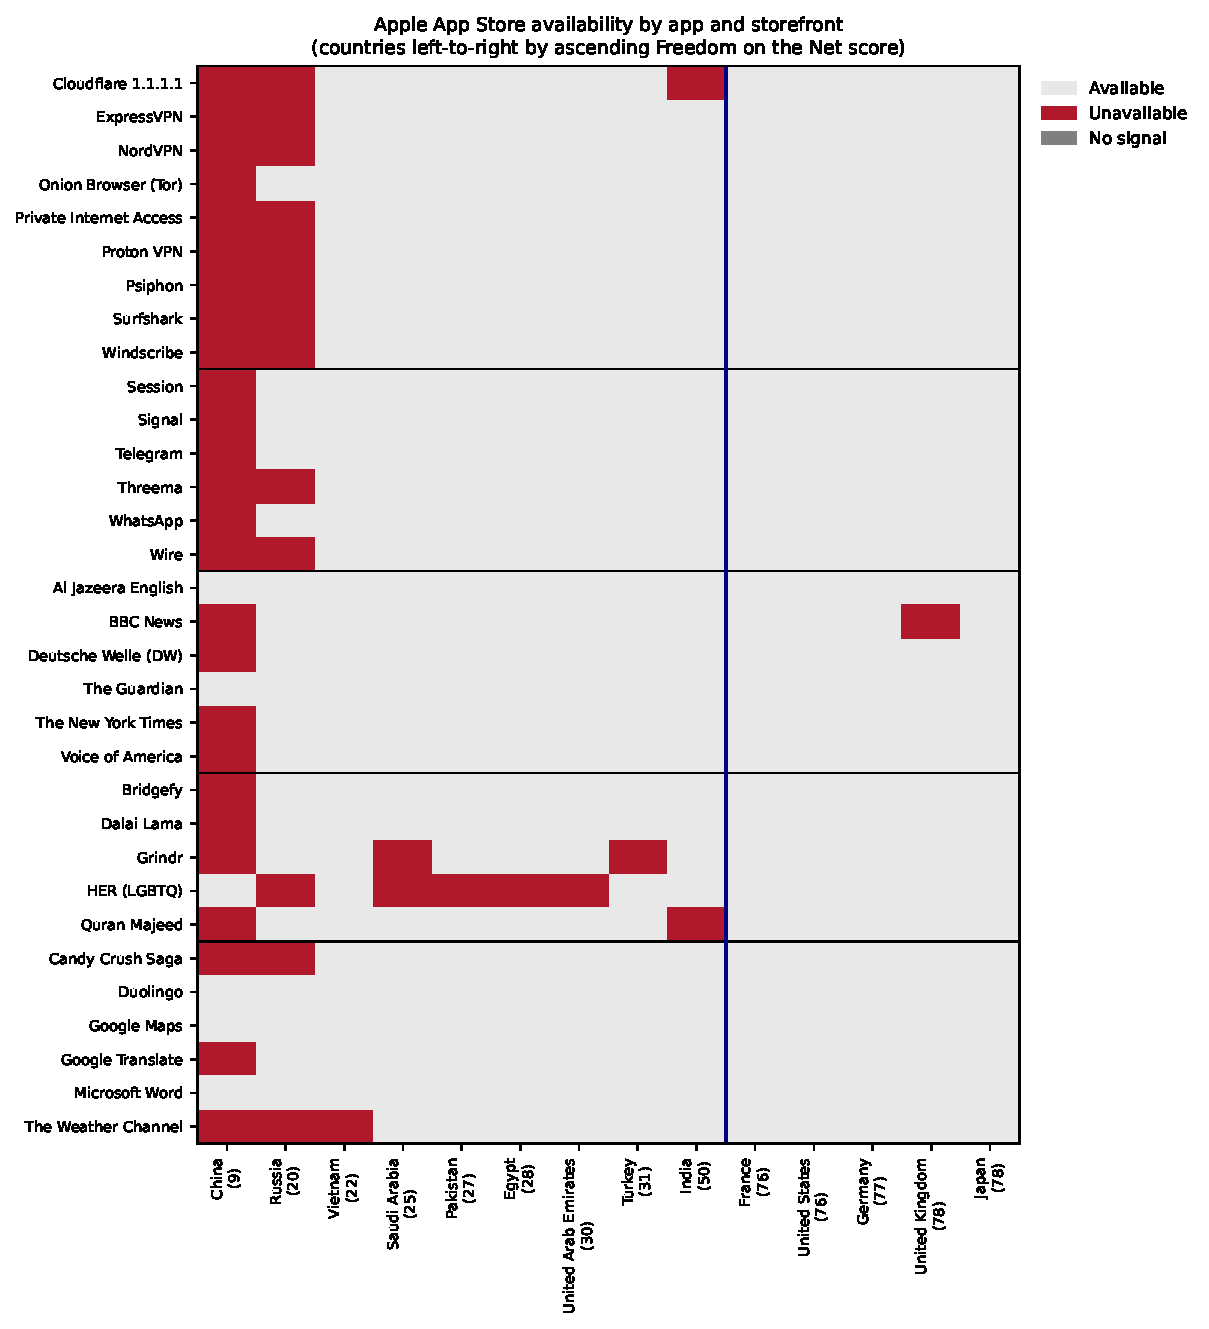
\includegraphics[width=\columnwidth]{figures/heatmap.pdf}
  \caption{Apple App Store availability for 32 apps across 14 national storefronts
  (snapshot of 23 July 2026). Red indicates the app is unavailable in that
  storefront. Rows are grouped by category; columns are ordered left-to-right by
  ascending \emph{Freedom on the Net} 2024 score, with the navy line separating
  known censors from free-expression baselines.}
  \label{fig:heatmap}
\end{figure}

\subsection{Validation Against Documented Events}

The snapshot independently reproduces every documented removal we tested. NordVPN
and Proton VPN are unavailable in Russia (the 2024 Roskomnadzor VPN
purge~\cite{techcrunch2024russia,moscowtimes2024russia}); NordVPN is unavailable in
China (the 2017 removals~\cite{cnbc2017china}); the \emph{New York Times} app is
unavailable in China (the 2017 removal); and Signal is unavailable in China. All
five checks pass, from raw availability data alone, which validates the method:
the pipeline surfaces known censorship without being told where to look.

\subsection{Cross-Country Pattern}

Censorship intensity is highly concentrated. Ranking countries by the share of
\emph{sensitive} apps (VPNs, messengers, news, topical) that are unavailable:

\begin{itemize}
  \item \textbf{China: 88.5\%} of sensitive apps missing (23 of 26 sensitive
  apps). Both the VPN and secure-messenger categories are \emph{entirely}
  removed (100\%), news is 67\% removed, and topical apps 80\%.
  \item \textbf{Russia: 42.3\%}, dominated by VPNs: 8 of 9 VPNs are gone, while
  messengers and news remain largely available. This is the signature of a
  targeted category action rather than a broad purge.
  \item \textbf{All other censors: $\leq 8\%$.} Saudi Arabia, Pakistan, Egypt, the
  UAE, and Turkey each remove only LGBTQ+ dating apps (Grindr and/or HER); India
  removes two apps (Cloudflare's 1.1.1.1 and a Quran app).
  \item \textbf{Baselines ($\leq 4\%$):} the US, France, Germany, and Japan show
  \emph{zero} sensitive removals; the UK shows one (discussed below).
\end{itemize}

\paragraph{Control normalization.} The neutral control apps bound the benign rate
of unavailability. In every baseline country the control-missing rate is 0\%, and
in the Gulf states, Turkey, Pakistan, Egypt, and India it is also 0\% while
sensitive apps are missing, so the sensitive removals there cannot be explained by
generic store churn. China is the exception: half its control apps are also missing
(Google Translate, The Weather Channel, Candy Crush), reflecting China's broad
blocking of Western services. Even there, the control-normalized excess (sensitive
minus control unavailability) is $+38.5$ points, the largest in the dataset.

\subsection{Correlation With Internet Freedom}

Per-country sensitive-app unavailability is negatively correlated with the
\emph{Freedom on the Net} 2024 score (Figure~\ref{fig:corr}): Pearson $r=-0.53$,
Spearman $r=-0.62$.

\begin{figure}[t]
  \centering
  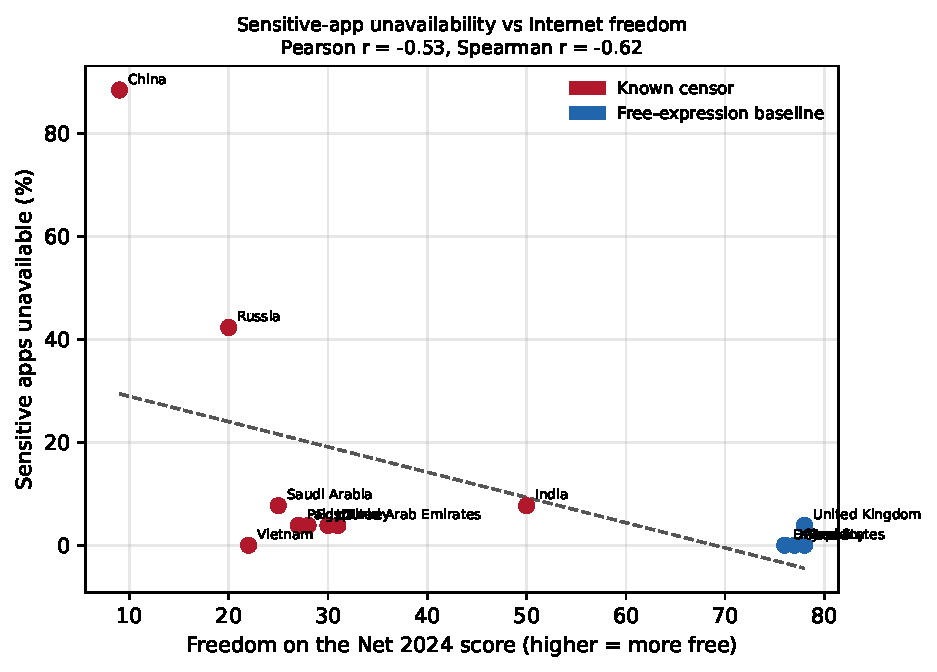
\includegraphics[width=\columnwidth]{figures/correlation.pdf}
  \caption{Per-country share of sensitive apps unavailable versus \emph{Freedom on
  the Net} 2024 score. Known censors (red) cluster at low freedom / high
  unavailability; baselines (blue) sit near zero. Pearson $r=-0.53$, Spearman
  $r=-0.62$.}
  \label{fig:corr}
\end{figure}

Less-free environments remove more sensitive apps. The
correlation is moderate rather than strong because the relationship is not linear:
a handful of severe censors (China, Russia) dominate, while most ``partly free''
countries remove only a single targeted category. This is itself a finding, app
store censorship is concentrated and category-specific, not a smooth function of a
country's overall repression score.

\subsection{Attribution: Where ``Missing'' Is Not ``Censored''}

Our data contains concrete cases that show why attribution must be explicit.

\paragraph{Sanctions-driven withdrawal (Russia).} Candy Crush and The Weather
Channel, two of our controls, are missing in Russia. These are almost certainly
\emph{developer} withdrawals tied to the post-2022 corporate exodus from Russia,
not state censorship. A naive availability count would misread them as repression;
our control track flags them as benign.

\paragraph{Regional app variants (UK).} The one ``removal'' in the UK is the
global \emph{BBC: World News \& Stories} app, which is not published in the UK
store because UK users receive a separate domestic BBC News app. This is a
methodological false positive from regional app variants, not censorship, and it
sets an upper bound on our precision that we report honestly.

\paragraph{Confidence labels.} Following Section~\ref{sec:eval}, we label China and
Russia's VPN/messenger removals \emph{documented} (they match transparency reports
and news), the Gulf/Turkey LGBTQ+ removals \emph{strongly inferred} (category-
consistent, control-clean, but not individually confirmed), and the India and
UK/Russia-control cases \emph{ambiguous} pending per-app confirmation.
